\section{Component Diagram}
\subsection{Sistema ServeEasy}
\subsubsection{single component del sistema}
\begin{figure}[H]
	\centering
	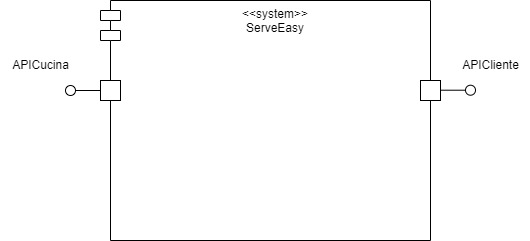
\includegraphics[scale=0.6]{iterazione1/images/ServeEasy_componente_unico.jpg}
	\caption{Component diagram - ServeEasy\label{fig:component_diagram_serveeasy}}
\end{figure}
Visualizzazione iniziale della soluzione come un componente unico che espone due API, dedicate rispettivamente alla cucina ed ai clienti. Si procede con uno sviluppo top-down.

\subsubsection{primo zoom-in sul sistema}

\begin{figure}[H]
	\centering
	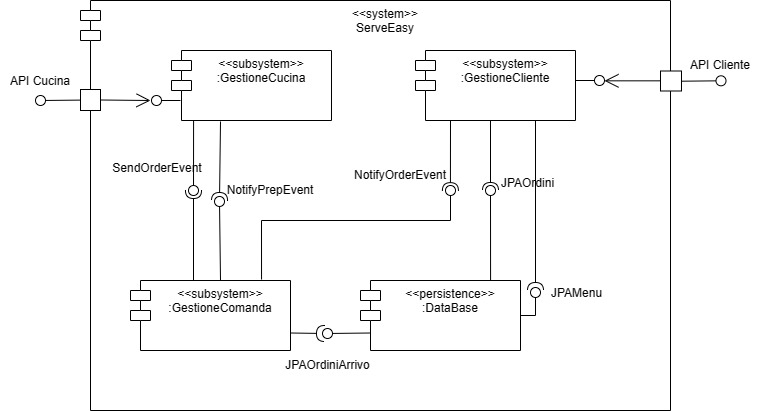
\includegraphics[scale=0.5]{iterazione1/images/ServeEasy_primo_zoomin.jpg}
	\caption{Component diagram - System\label{fig:component_diagram_system}}
\end{figure}
Al primo zoom-in si identificano i servizi che andranno a comporre l’architettura della soluzione:
\begin{itemize}
	\item \textbf{GestioneComanda:} risolve gli use case del gruppo “sistema”, rappresenta il cuore del sistema ed incorpora la logica di backend fondamentale per la gestione regolarizzata degli ordini da cliente a cucina, attraverso politiche di schedulazione a priorità progettate ed implementate con un algoritmo ad-hoc.
	\item \textbf{GestioneCliente:} risolve gli use case del gruppo “cliente”, espone le funzionalità destinate ai dispositivi di tavolo ed al portale web per clienti d’asporto. Ha dunque il compito di gestire gli aspetti del servizio legati alle interazioni del cliente col sistema, come la visualizzazione del menu, la creazione degli ordini ed il raggruppamento degli ordini in una comanda relativa.
	\item \textbf{GestioneCucina:} risolve gli use case del gruppo “cucina”, espone le chiamate destinate ai dispositivi di cucina. Questo servizio conterrà un sistema a code, dove l’ordine in arrivo verrà classificato ed inserito in base al suo ingrediente principale. Gli ordini verranno gestiti dalle postazioni della cucina seguendo una politica FIFO.
\end{itemize}
Per la memorizzazione persistente dei dati cruciali per l’attività come piatti, ordini e comande, è stato inserito un componente database.
All’interno del sistema ServeEasy, i componenti comunicano tra loro attraverso una comunicazione ad eventi, asincrona. Si è deciso di attuare una politica pub-sub per la gestione delle comunicazioni interne, costituite da scambi di notifiche e DTO tra i microservizi designati.

\subsection{Gestione Comanda}
\subsubsection{Componenti esagonali}
Il design dei microservizi seguirà l’architettura esagonale: un dominio, denominato “Domain”, nucleo della logica di servizio, sarà racchiuso tra due gusci denominati “Interface” e “Infrastructure”, i quali avranno il compito di astrarre la gestione dati, rendendola opaca al dominio. La logica di base del microservizio seguirà lo schema port-adapter, dove il dominio comunica con i gusci attraverso delle interfacce dette porte (il cui nome nel progetto è caratterizzato dal suffisso “Port”), mentre i gusci hanno il compito di implementare l’effettivo componente di trasmissione (guscio Infrastructure) e/o ricezione (guscio Interface), detto adattatore (sarà identificabile da suffisso “Adapter”). 
Nello specifico il \textbf{Domain} definisce gli oggetti, le entità e le operazioni che sono pertinenti al problema che il microservizio gestisce.Gli \textbf{Interface adapters} fungono da ponte tra il mondo esterno e il core del sistema, consentendo al microservizio di comunicare con altre applicazioni, servizi o dispositivi esterni in modo indipendente dall'implementazione interna del sistema stesso, mentre gli \textbf{Infrastructure adapters} fungono da ponte tra il core del sistema e l'infrastruttura esterna, gestendo le chiamate e le operazioni necessarie per accedere e utilizzare le risorse infrastrutturali.
Tali caratteristiche avvantaggiano l’intercambiabilità dei singoli componenti di sistema a costo di un aumento della complessità.
\begin{figure}[H]
	\centering
	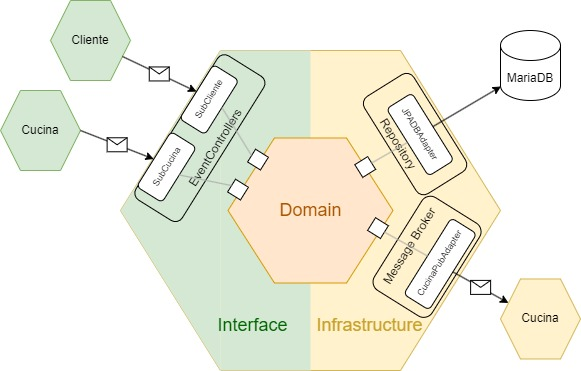
\includegraphics[scale=0.7]{iterazione1/images/hexagon.jpg}
	\caption{Architettura esagonale per il microservizio Gestione comanda\label{fig:hexagon}}
\end{figure}

\subsubsection{zoom-in gestione comanda}
\begin{figure}[H]
	\centering
	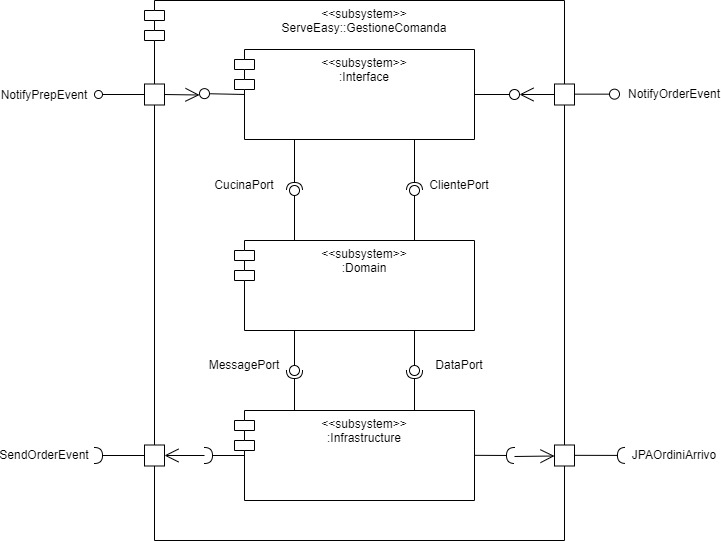
\includegraphics[scale=0.5]{iterazione1/images/component_comanda_cucina-GestioneComanda.jpg}
	\caption{Component diagram - Gestione Comanda\label{fig:component_diagram_gestione_comanda}}
\end{figure}


\subsubsection{zoom-in infrastructure di gestione comanda}
\begin{figure}[H]
	\centering
	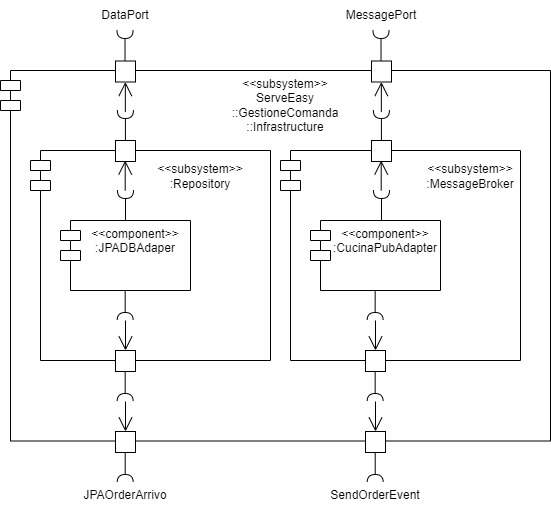
\includegraphics[scale=0.5]{iterazione1/images/component_comanda_cucina-GestioneComanda__Infrastructure.jpg}
	\caption{Component diagram - Gestione Comanda - Infrasrtructure \label{fig:component_diagram_gestione_comanda_infrastracture}}
\end{figure}
\begin{itemize}
    \item Repository: JPADBAdapter per la comunicazione con il database;
    \item MessageBroker: CucinaPubAdapter per l'invio di messaggi sul topic verso il microservizio della cucina.
\end{itemize}

\subsubsection{zoom-in domain di gestione comanda}
\begin{figure}[H]
	\centering
	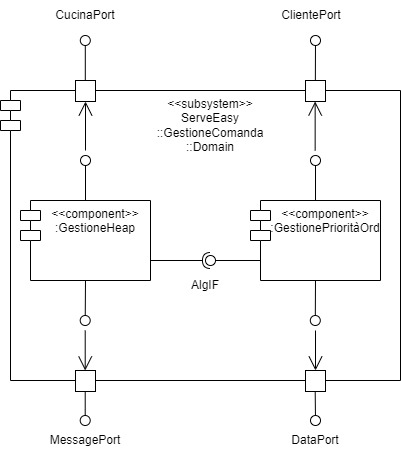
\includegraphics[scale=0.5]{iterazione1/images/component_comanda_cucina-GestioneComanda__Domain.jpg}
	\caption{Component diagram - Gestione Comanda - Domain \label{fig:component_diagram_gestione_comanda_domain}}
\end{figure}

\subsubsection{zoom-in interface di gestione comanda}
\begin{figure}[H]
	\centering
	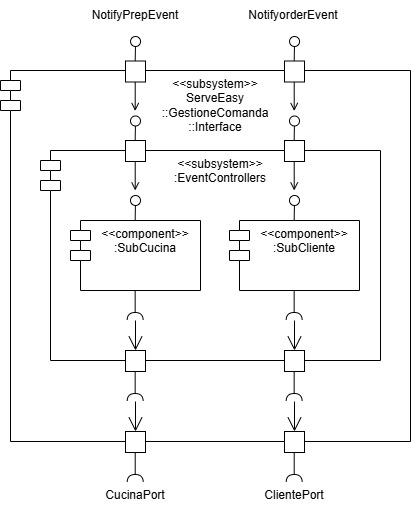
\includegraphics[scale=0.5]{iterazione1/images/component_comanda_cucina-GestioneComanda__Interface.jpg}
	\caption{Component diagram - Gestione Comanda - Interface \label{fig:component_diagram_gestione_comanda_interface}}
\end{figure}
\begin{itemize}
    \item EventControllers: SubCucina e SubCliente, permettono la ricezione di messaggi tramite message broker dagli altri microservizi.
\end{itemize}

\subsection{Gestione Cliente}
\subsubsection{zoom-in gestione cliente}
\begin{figure}[H]
	\centering
	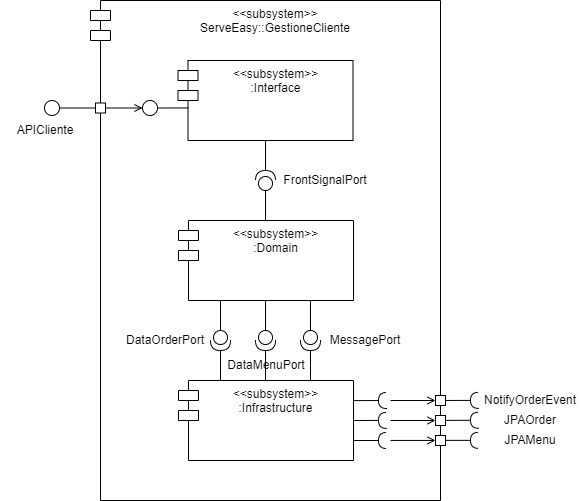
\includegraphics[scale=0.5]{iterazione1/images/GestioneCliente_subsystem-GestioneCliente.jpg}
	\caption{Component diagram - Gestione Cliente \label{fig:component_diagram_gestione_cliente}}
\end{figure}

\subsubsection{zoom-in infrastructure di gestione cliente}
\begin{figure}[H]
	\centering
	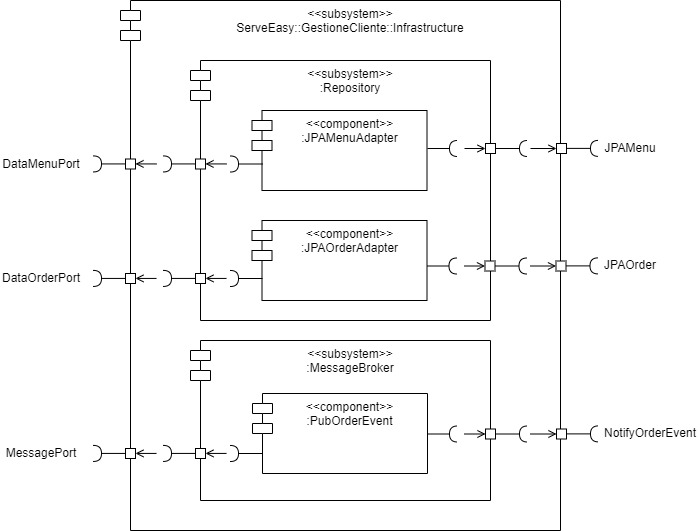
\includegraphics[scale=0.5]{iterazione1/images/GestioneCliente_subsystem-Infrastructure.jpg}
	\caption{Component diagram - Gestione Cliente - Infrastructure \label{fig:component_diagram_gestione_cliente_infrastructure}}
\end{figure}
\begin{itemize}
    \item Repository: JPAOrderAdapter e JPAMenuAdapter per la comunicazione con il database;
    \item MessageBroker: PubOrderEvent per l'invio di messaggi sul topic verso il microservizio della cucina.
\end{itemize}

\subsubsection{zoom-in domain di gestione cliente}
\begin{figure}[H]
	\centering
	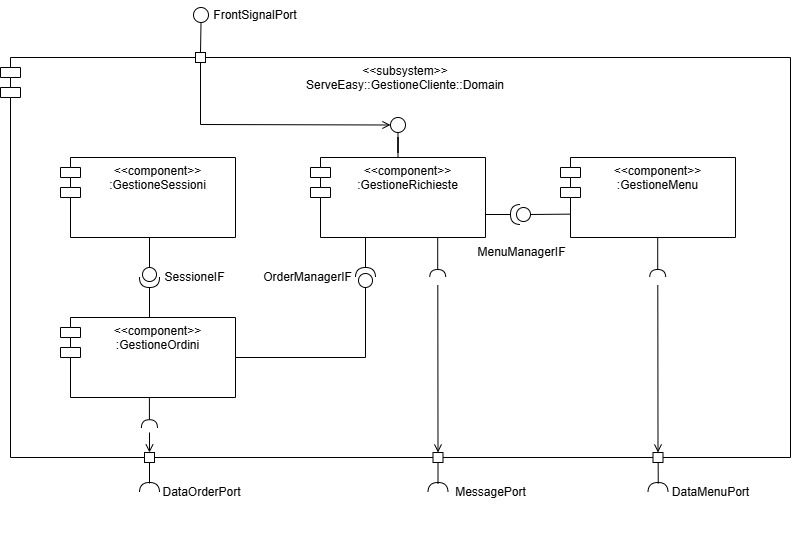
\includegraphics[scale=0.5]{iterazione1/images/GestioneCliente_subsystem-Domain.jpg}
	\caption{Component diagram - Gestione Cliente - Domain \label{fig:component_diagram_gestione_cliente_domain}}
\end{figure}

\subsubsection{zoom-in interface di gestione cliente}
\begin{figure}[H]
	\centering
	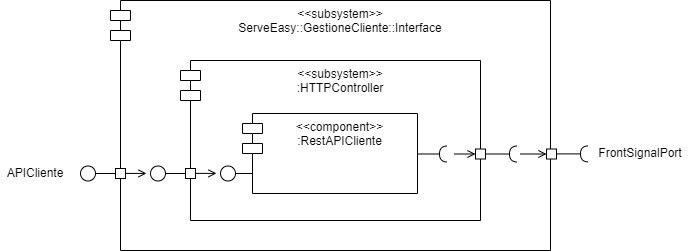
\includegraphics[scale=0.5]{iterazione1/images/GestioneCliente_subsystem-Interface.jpg}
	\caption{Component diagram - Gestione Cliente - Interface \label{fig:component_diagram_gestione_cliente_interface}}
\end{figure}
\begin{itemize}
    \item HTTPControllers: RestApiCliente, permette di esporre API verso l'esterno.
\end{itemize}

\subsection{Gestione Cucina}
\subsubsection{zoom-in gestione cucina}
\begin{figure}[H]
	\centering
	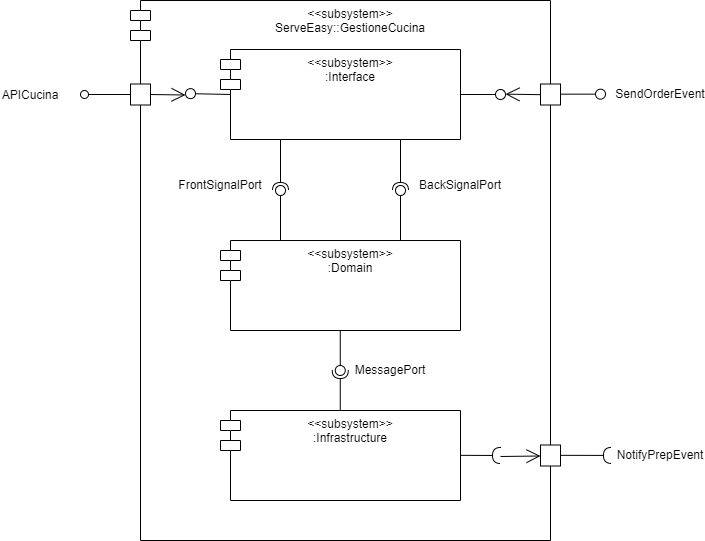
\includegraphics[scale=0.5]{iterazione1/images/component_comanda_cucina-GestioneCucina.jpg}
	\caption{Component diagram - Gestione Cucina \label{fig:component_diagram_gestione_cucina}}
\end{figure}

\subsubsection{zoom-in infrastructure di gestione cucina}
\begin{figure}[H]
	\centering
	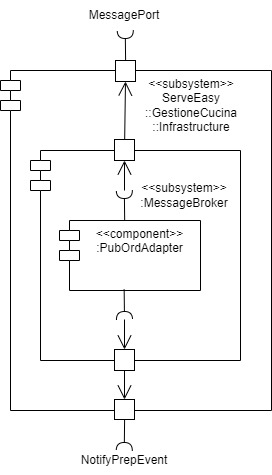
\includegraphics[scale=0.5]{iterazione1/images/component_comanda_cucina-GestioneCucina__Infrastructure.jpg}
	\caption{Component diagram - Gestione Cucina - Infrastructure \label{fig:component_diagram_gestione_cucina_infrastructure}}
\end{figure}
\begin{itemize}
    \item Repository: JPADBAdapter per la comunicazione con il database;
    \item MessageBroker: PubOrderAdapter per l'invio di messaggi sul topic verso il microservizio di GestioneComanda.
\end{itemize}

\subsubsection{zoom-in domain di gestione cucina}
\begin{figure}[H]
	\centering
	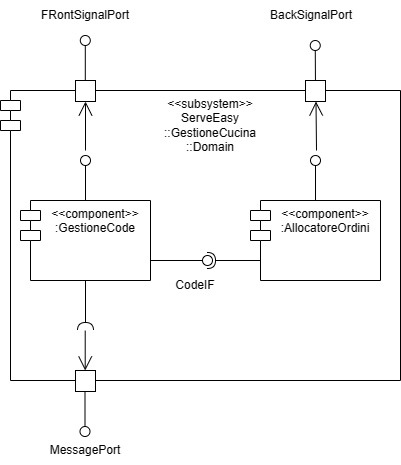
\includegraphics[scale=0.5]{iterazione1/images/component_comanda_cucina-GestioneCucina__Domain.jpg}
	\caption{Component diagram - Gestione Cucina - Domain \label{fig:component_diagram_gestione_cucina_domain}}
\end{figure}

\subsubsection{zoom-in interface di gestione cucina}
\begin{figure}[H]
	\centering
	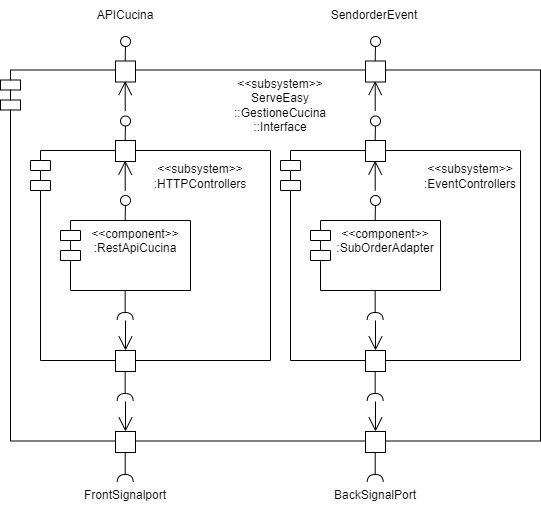
\includegraphics[scale=0.5]{iterazione1/images/component_comanda_cucina-GestioneCucina__Interface.jpg}
	\caption{Component diagram - Gestione Cucina - Interface \label{fig:component_diagram_gestione_cucina_interface}}
\end{figure}
\begin{itemize}
    \item EventControllers: SubOrderAdapter, permette la ricezione di messaggi tramite message broker dal microservizio GestioneComanda;
    \item HTTPControllers: RestApiCucina, permette di esporre API verso l'esterno.
\end{itemize}



\clearpage